\documentclass[a4paper,11pt]{scrreprt}                       % default is A4 paper style and 11pt font size


%%%%%%%%%%%% version history %%%%%%%%%%%%%%%%%%%%%%%%%%%%%%%%%%%

%26.03.2017:    corrections for the latex source-code: diacritics issues; corrected the glossaries and added listings packages; added fontspec (only works with xelatex/lualatex !!!)
%2014:          put in latex version + some small additions - Florin Stoican
%2013:          content from Dan Stefanoiu
%%%%%%%%%%%%%%%%%%%%%%%%%%%%%%%%%%%%%%%%%%%%%%%%%%%%%%%%%%%%%%%%%%%%%%%%%


%%%%%%%%%%%% macros for various paths %%%%%%%%%%%%%%%%%%%%%%%%%%%%%%%%%%%
\def \cls {./cls} 																					 % path to common latex files (change for your own relative/absolute path)
\def \pics {./pics}      																		 % path to pics files (change for your own relative/absolute path)
\def \chapters {./chapters}      														 % path to chapter files (change for your own relative/absolute path)
\def \code {./code}      													        	 % path to source code files (change for your own relative/absolute path)

% you don't have to use them but it's nicer this way
%%%%%%%%%%%%%%%%%%%%%%%%%%%%%%%%%%%%%%%%%%%%%%%%%%%%%%%%%%%%%%%%%%%%%%%%%

% language={english/romanian} selects between the languages used in the manusript (changes, e.g., the name of the chapter)
% type={bachelor/master/phd} selects between the type of manusript (changes, e.g., the titlepage make-up)
\usepackage[language=romanian,type=bachelor]{\cls/standard} % introduces useful packages and commands(CHANGE ONLY IF YOU KNOW WHAT YOU'RE DOING)
\addbibresource{\cls/bib.bib}																% bib resource (using biblatex package, for complex stuff use the biber backend instead of bibtex
\newglossaryentry{computer}
{
  name=computer,
  description={is a programmable machine that receives input,
               stores and manipulates data, and provides
               output in a useful format}
}

\newacronym[longplural={Frames per Second}]{fpsLabel}{FPS}{Frame per Second}
\newacronym{lvm}{LVM}{Logical Volume Manager}        																	% put here all your glossary terms; only the ones actually used will appear in the glossary list of the manuscript

\begin{document}

%%%%%%%%%%%%%%%%%%%%%%% frontmatter %%%%%%%%%%%%%%%%%%%%%%%%%%%%%%%%%%%%%
\pagenumbering{roman}																				% default numbering for the frontmatter is roman

\title{Clasificare defecte într-o rețea de apă de mari dimensiuni}														% title of your manuscript
\author{Cazan Cristian-Claudiu}																				% author name
\advisor{Florin Stoican}																			% advisor name

\maketitle

% show table of contents, figures, tables and algorithms

\tableofcontents 
\printnoidxglossaries																				% \printglossaries works only if the makeindex has the correct arguments
\addcontentsline{toc}{chapter}{\listfigurename}
\listoffigures 
\addcontentsline{toc}{chapter}{\listtablename}
\listoftables
\addcontentsline{toc}{chapter}{\listalgorithmcfname}
\listofalgorithmes

\clearpage

%%%%%%%%%%%%%%%%%%%%%%% mainmatter %%%%%%%%%%%%%%%%%%%%%%%%%%%%%%%%%%%%%%
\pagenumbering{arabic}																			% default numbering for the mainmatter is arabic

% here is the text of you manuscript; you can put it directly here but it is better to include files (the main file will be more compact)
\chapter{Introducere}
\label{chap:intro}

\section{Motivația alegerii temei}
Transportul și distribuția apei reprezintă una dintre cele mai vechi preocupări inginerești de proporții, existând de mai mult de 4000 de ani. Civilizația minoică, localizată în insula Creta, este considerată a fi prima care a construit apeducte - structuri pentru transportul apei de la sursă către orașe - în 2500 î.Hr. 

Deși majoritatea popoarelor din antichitate care s-au ocupat cu construcția apeductelor întrebuințau aceste sisteme pentru irigația pământului - ocupațiile de bază de atunci fiind în strânsă legătură cu agricultura - romanii au văzut în sistemele de provizionare a apei și un potențial imens în dezvoltarea civilizației, astfel ei sunt ei care aduc cele mai mari contribuții inginerești, apeductele construite de aceștia impresionând și astăzi prin grandoarea și iscusunța cu care au fost construite.

Inovațiile în acest domeniu au suferit salturi bruște și puternice în momentul descoperirii unei noi relații matematice care transformă un parametru despre care se puteau face doar niște estimări grosiere într-o mărime bine definită și bine controlată. Istoric vorbind începutul dezvoltării științei hidraulice s-a bazat pe relația descoperită de Arhimede din Siracuza în sec III î.Hr, $F = V_{obiect} \cdot \rho_{lichid}*g$. O altă contribuție care are o deosebită importanță în domeniul tehnologiei de distribuiție a apei și nu numai o reprezintă tubul lui Pitot folosit la măsurarea vitezei fluidului, inventat de Henri Pitot în sec XVII. Din punct de vedere constructiv tubul are o formă de \textbf{L}, scufundarea acestuia într-un fluid (apă sau gaz) va determina creșterea nivelului și a presiunii până la o anumită limită \cite{klopfenstein1998air}, ecuația care guvernează depedența nivel - viteză este:
\begin{equation}
u = \sqrt{\frac{2(p_t-p_s)}{\rho}} 
\end{equation}

unde:

\begin{description}
\item u reprezintă viteza fluidului;
\item $p_t$ reprezintă presiunea de stagnare;
\item $p_s$ reprezintă presiunea statică;
\item $\rho$ reprezintă densitatea fluidului.
\end{description}

Mergând mai departe, alte contribuții importante apar din partea marilor matematicieni precum Daniel Bernoulli și Leonhard Euler, care au mărit spectrul mecanicii lui Newton și Leibniz spre aria hidraulicii și a termodinamicii. Fluidele considerate sunt incompresibile și au densitatea constantă în timp și uniform distribuită în spațiu. Bernoulli afirmă despre lichidele incompresibile că o creștere în viteză a lichidului este însoțită de o scădere a energiei potențiale a lichidului (i.e. a presiunii):
\begin{equation}
\frac{u^2}{2} + gz + \frac{p}{\rho} = c
\end{equation}

unde:
\begin{description}
\item v reprezintă viteza fluidului;
\item g reprezintă accelerația la care e supus fluidul;
\item z reprezintă elevația ștrangulației conductei;
\item p reprezintă presiunea într-un anumit punct;
\item $\rho$ reprezintă densitatea fluidului.
\end{description}

În contextul în care se dorește analiza unui caz real este important ca toate diferențele între cazurile ideale și cazurile reale să fie puse în evidență în mod matematic, astfel se particularizează ecuația generală Navier-Stokes pentru cazuri în care se cunosc anumiți parametrii ai sistemului de analizat. Spre exemplu ecuația Poisuille care modelează începutul fluxului de apă într-o conductă este \cite{elger2016engineering}:
\begin{equation}
\frac{\partial u}{\partial t} = \frac{G}{\rho} + \nu \left( \frac{\partial^2 u}{\partial t^2} + \frac{1}{r}\frac{\partial u}{\partial{r}}\right)
\end{equation}

unde:
\begin{description}
\item $u$ reprezintă viteza lichidului prin conductă
\item $t$ reprezintă timpul
\item $G$ reprezintă diferența de presiune
\item $\rho$ reprezintă densitatea lichidului
\item $\nu$ reprezintă vâscozitatea cinematică
\item $r$ reprezintă poziția
\end{description}

Se poate observa că pe măsură ce modelul matematic se apropie de realitate, complexitatea acestuia crește și pentru fiecare situație specială - spre exemplu analiza presiunii la  introducerea apei într-o conductă vs. analiza presiunii când conducta este încărcată cu apă - are nevoie de o ecuație specială sau de o particularizare a ecuației Navier-Stokes, pentru care încă nu se cunoaște dacă există soluții pentru cazul cu 3 dimensiuni și dacă soluțiile acestea sunt netede. 

Ținând cont de importanța apei în desfășurarea activităților cotidiene atât pentru oameni cât și pentru actorii importanți ai industriei, este o condiție absolut necesară ca un oraș să aibă un sistem performant de distribuție a apei. În contextul actual al dezvoltării tehnologiei este natural să folosim tehnici moderne de monitorizare a diferiților parametrii din cadrul unei rețele pentru a putea face o analiză riguroasă și eficientă cu referire nu numai la mentenanță ci și la consumul global și local în ideea îmbunătățirii și reducerii pierderilor.


\section{Expunerea problemei}

În această lucrare se va aborda problematica identificării prezenței unui defect - \textit{Fault detection} și izolarea defectului \textit{Fault isolation} apărut într-un nod al rețelei - aceasta reprezentând o simplificare deoarece un defect apare de obicei într-una din conductele rețelei legate de acel nod. Combinănd cei doi termeni obținem \textit{Fauld detection and Isolation} (FDI).

O rețea de apă poate fi privită ca un graf neorientat $G = (V, E)$ unde $V$ este mulțimea nodurilor rețelei - acestea reprezentând o abstractizare asupra componentelor precum:
\begin{itemize}
\item rezervoare
\item tancuri de apă
\item puncte de distribuție
\end{itemize} 

$E$ este mulțimea muchiilor reprezentând de fapt țevile care fac legătura între noduri.

Mergând mai departe cu abstractizarea se pot considera rețele de apă active și rețele de apă pasive. Diferența între cele două făcându-se în baza pompelor de apă amplasate în zonele unde presiunea sau elevația vin în detrimentul distribuției apei.

Rețelele de apă care vor fi tratate în această lucrare fac parte din categoria pasivă, astfel putem diviza mulțimea nodurilor $V$ în $V^t$ și în $V^j$ reprezentând mulțimea nodurilor de tip tanc și mulțimea nodurilor joncțiune, cu proprietatea că $V = V^t \cup V^j$. Tancurile și rezervoarele dintr-o rețea de apă au proprietatea că nivelul de apă din acestea se va menține la un nivel oarecum staționar, astfel simulările din capitolele viitoare se vor axa pe nodurile simple de tip joncțiune, deci mulțimea de interes în acest caz va fi $V^j$ pentru care cunoaștem cardinalul.

Caracteristicile care se pot recolta dintr-o rețea de apă pot varia în funcție de elementul inspectat și de senzorii dispuși în rețea, astfel pentru fiecare nod $n_i \in V^j$ putem defini la fiecare moment de timp 
\begin{itemize}
\item presiunea $p_i(t)$ - măsurată în metri coloană de apă $mH2O$, mărime influențată puternic de presiunea interioară a nodului și de eventualele perturbații exterioare i.e. scurgeri de apă prin conducte;
\item 'cererea' $d_i(t)$ - măsurată $L/s$, mărime ce caracterizează profilul de utilizare al utilizatorilor de-a lungul unei zile i.e. debitul de apă care ajunge la consumatori. Acest debit poate varia de-a lungul zilei, putem distinge de exemplu intervale de timp în care cererea este foarte mică și rețeaua intră în regim staționar;
\item de asemenea pentru fiecare conductă a rețelei $e_{ij} \in E$ putem măsura viteza lichidului $v_{ij}(t)$.
\end{itemize}



Pentru a putea rezolva problema de FDI este importantă găsirea unei modalități eficiente de selecție și prelucrare a datelor de la rețea.Mai mult, punând în lumină aspectul ingineresc al problemei, trebuie găsită o submulțime $V_{opt} \subset V^j$ ai cărei elemente pot aduce informații necesare și suficiente pentru a detecta un defect într-o acoperire destul de mare a rețelei.

\section{Exemplul de lucru}
În următoarele capitole și în implementarea lucrării consider rețeaua Hanoi iar pentru simularea scenariilor propuse voi folosi biblioteca și suita de funcții \textbf{EPANET} - Environmental Protection Agency NETwork \cite{rossman2000epanet}. 

\noindent Rețeaua Hanoi constă într-o mulțime de noduri de tip joncțiune $V^j$ cu $|V^j| = 31$ și mulțimea $V^t$ cu $|V^t|=1$, ilustrată în figura de mai jos:
 
\begin{figure}[h]
\centering
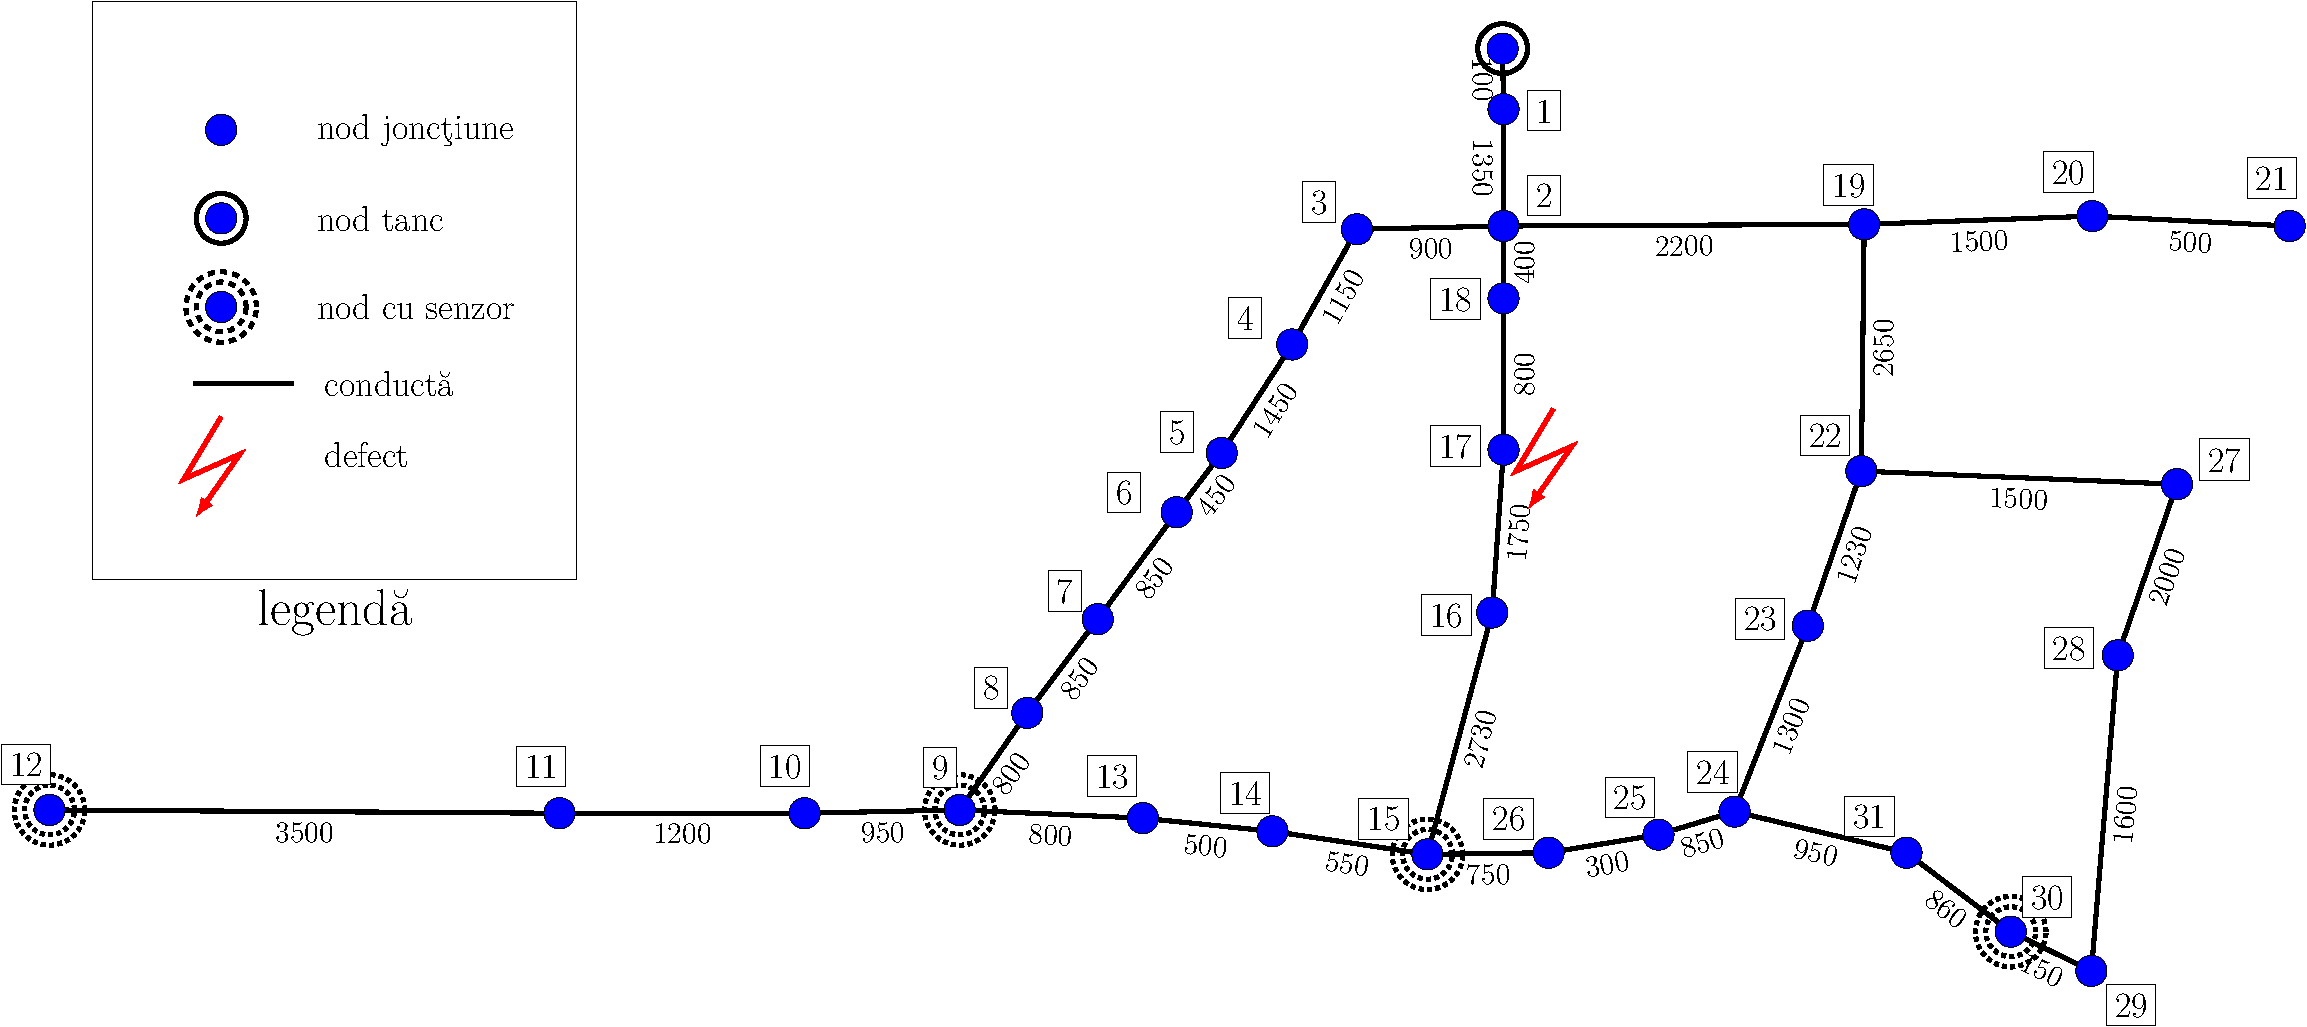
\includegraphics[width=\textwidth]{pics/c1_pics/hanoi_network.pdf}
\caption{Graful rețelei de apă din Hanoi \cite{irofti2017dictionary}}
\label{fig:hanoinetwork}
\end{figure}

După cum se poate observa în figura de mai sus au fost reprezentate două tipuri de node pasive, anume tancurile și joncțiunile. În cazul apariției unui defect în rețea, este important de luat în considerație modalitatea în care acesta va influența valorile apărute în rețea, spre exemplu este de la sine înțeles că dacă se cosideră un defect în nodul cu indicele 17 - i.e. în acest nod au apărut anumite scurgeri care afectează fluxul de apă către consumatori - nodurile în care se va observa o modificare puternică a caracteristicilor (presiune și debit) vor face parte din mulțimea nodurilor adiacente rețelei $S=\{V_{16}, V_{18}\}$, deși pare o concluzie naturală, o modelare matematică riguroasă din care să se tragă această nu este o problemă ușor de rezolvat, anumiți parametrii fiind extrem de greu de estimat chiar și în cazul în care se consideră un regim staționar.

%\chapter{Despre plagiat}
\label{chap:div}


\myLettrine{C}{onform} Dicţionarului Explicativ al Limbii Române:

\blockquote{PLAGIA: A-şi însuşi, a copia total sau parţial ideile, operele etc. cuiva, prezentându-le drept creaţii personale; a comite un furt literar, artistic sau ştiinţific.}

	În contextul lucrărilor ştiinţifice, plagiatul îl reprezintă utilizarea ideilor, tehnologiilor, rezultatelor sau textelor altor persoane, fie prin omiterea referirii lucrării originale, fie prin însuşirea acestora. Pentru evitarea plagiatului se recomandă menţionarea sursei (şi implicit a autorului sau autorilor originali) unei idei, teorii, a unor fapte statistice care nu ţin de cultura generală, citate ale altor autori (fie scrie sau vorbite), parafraze.

	Se recomandă includerea între ghilimele a secţiunilor de text citate din alte opere (exemplu mai sus), cu menţionarea sursei. De asemenea, în cazul parafrazelor, nu este de ajuns doar schimbarea a câteva cuvinte, ci este necesară o re-interpretare a textului original în viziunea autorului lucrării în care se foloseşte parafraza. Şi în acest caz este necesară menţionarea sursei.

	În România, legea drepturilor de autor este \textbf{Legea nr. 8/1996} completată de \textbf{Legea nr. 285 din 23 iunie 2004} şi \textbf{Ordonanţa de urgenţă 123 din 1 septembrie 2005}.


%\chapter{Detalii formatare \LaTeX}
\label{chap:main}

\myLettrine{M}{aterialul} curent folosește ca template clasa \textquote{scrrprt} la care s-au adăugat pachete și comenzi uzuale. 

\shadowbox{
\begin{minipage}{.95\textwidth}
Datorită folosirii pachetului \emph{fontspec} ce acceptă în mod nativ diacritice, fișierul sursă latex se poate compila doar cu \textbf{xelatex}, nu și cu \textbf{pdflatex}.
\end{minipage}
}

Pentru a păstra o structură cât mai compactă fișierele sursă s-au împărțit în următoarele categorii\footnote{Nu este obligatoriu să se păstreze aceeași structură dar este recomandat, pentru a păstra o formatare compactă.}:
\begin{description}[style=nextline]
\item[thesis.tex] reprezintă fișierul \textquote{main} în care toate celelalte fișiere sunt apelate
\item[standard.sty] conține pachetele și comenzile folosite uzual
\item[bib.bib] conține câteva referințe în format \emph{bibtex}; referințe adiționale pot fi adăugate după necesități \url{https://texblog.org/2014/04/22/using-google-scholar-to-download-bibtex-citations/}
\item[upb-authoryear.bbx, upb-authoryear.cbx si romanian.lbx] definesc stilul bibliografic asociat intrărilor din lista bibliografică
\item[gls.tex] conține termeni de glosar ce pot fi adăugați la o \textquote{Listă de termeni} dacă se consideră necesar
\end{description}
Comentarii și scurte explicații (în engleză) referitor la rolul pachetelor și comenzilor se regasesc în aceste fișiere sursă.

Adițional, următoarea structură de dosare a fost folosită:
\begin{description}[style=nextline]
\item[cls] pentru stocarea fișierelor-sursă auxiliare (pentru introducerea de pachete/referințe bibliografice, etc.)
\item[pics] pentru stocarea imaginilor ce vor fi adaugate în manuscris
\item[chapters] pentru stocarea fișierelor \textquote{capitol} (pentru ușurința în lucru, am presupus că textul fiecărui capitol va fi pus într-un fișier sursă de sine-stătător)
\item[code] pentru stocarea fișierelor \textquote{sursă} ce vor fi apoi adăugate în manuscris
\end{description}

\begin{rem}
\label{rem:at}
În cazul în care se dorește modificarea structurii mai sus-menționate, o atenție sporită trebuie acordată referințelor făcute în cadrul fișierelor. \eor
\end{rem}

Fișierele au fost compilate folosind distribuția Miktex 2.9 (\url{http://miktex.org/2.9/setup}), cu ajutorul editorului de text TexnicCenter (\url{http://www.texniccenter.org/}). Detalii generale despre \LaTeX se pot găsi de exemplu în \url{http://tobi.oetiker.ch/lshort/lshort.pdf}. În cele ce urmează sunt prezentate câteva situații tipice.


\section{Exemple comenzi de tip float}
În această secțiune  vor fi exemplificate câteva construcții de tip \textquote{float}. În general, fiecărui float i se poate asocia un element de tip \emph{legendă} pentru a putea da o explicație detaliată și un element de tip \emph{etichetă}, ce va permite referirea la acest float în cadrul manuscrisului cât și enumerarea sa în cadrul listei asociate (de exemplu in \emph{lista de figuri} vor apare toate figurile definite în manuscris).

\subsection{Tabele}
Informații suplimentare despre tabele pot fi gâsite de exemplu în \url{http://en.wikibooks.org/wiki/LaTeX/Tables}.
Câteva exemple simple sunt ilustrate în continuare.

\begin{table}[ht!]
\begin{tabular}{llll}
\hline
Fault & Fault & Symbol & Type\\ 
No. & & & \\
\hline
1 & Sensor Fault & $\Delta\beta_{1,m1}$ & Fixed Value\\
2 & Sensor Fault & $\Delta\beta_{2,m2}$ & Gain Factor\\
3 & Sensor Fault & $\Delta\beta_{3,m1}$ & Fixed Value\\
4 & Sensor Fault & $\Delta\omega_{r,m1}$ & Fixed Value\\
5 & Sensor Fault & $\Delta\omega_{r,m2}$, $\Delta\omega_{g,m2}$ & Gain Factor\\ 
\hline
\end{tabular}
\centering
\caption{Faults affecting the wind turbine model}%Considered Faults}
\label{tab:faults}
\end{table}

\begin{table}[ht!]
\begin{center}
\begin{tabular}{|c|c|c|c|c|c|c|c|}
\hline
no. of hyperplanes&5&10&15&20&25&50&100\\ \hline
classical&9.91&64.06&91.74&511.47&306.04&$\cdots$&$\cdots$\\ \hline
enhanced&1.14&0.81&0.59&4.84&4.18&3.66&2.94\\ \hline
\end{tabular}
\end{center}
\caption{Numerical values for the solving of an MI optimization problem under classical and anhanced methods.}
\label{tab:run}
\end{table}

Atât \tabref{tab:faults} cât și \tabref{tab:run} vor aparea în lista de tabele și vor putea fi referite în text cu ajutorul etichetei asociate fiecăruia.

\subsection{Figuri}
În mod similar se pot afișa diverse imagini (se recomandă fie imagini în format raster de rezoluție suficientă, fie imagini in format vectorial -- eps, pdf, tikz). Detalii suplimentare se pot găsi de exemplu în \url{http://en.wikibooks.org/wiki/LaTeX/Floats,_Figures_and_Captions}.

\begin{figure}[!ht]
\begin{center}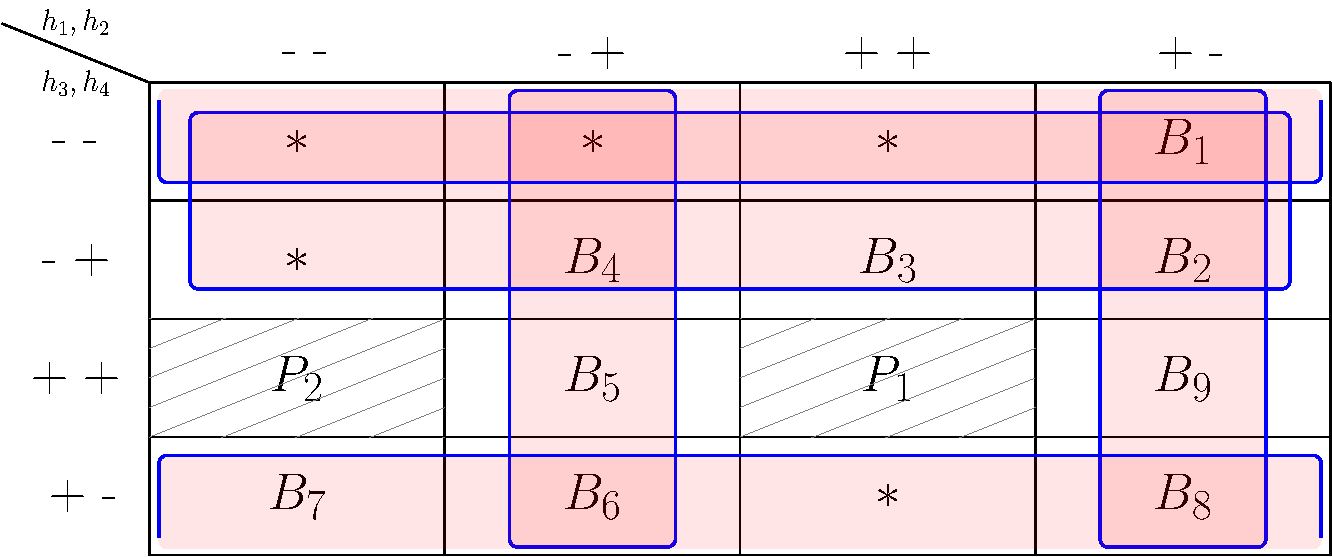
\includegraphics[width=\singlefigure]{\pics/binary/KarnaughDiagramForHyperplaneArrangement}\end{center}
	\caption{Karnaugh diagram for obaining the reduced cell representation}
	\label{fig:karnaugh}
\end{figure}

În \figref{fig:karnaugh} se ilustrează un exemplu simplu (o singură figură) iar în \figref{fig:int} se face uz de pachetul \textquote{subfig} ce permite o structură de tip tabel cu mai multe sub-figuri (fiecare dintre acestea poate fi referită în mod independent -- de exemplu, \figref{fig:int}\subref{fig:intc}).

\begin{figure}[!ht]
\begin{center}
  \subfloat[cut for each tuple]{\label{fig:inta}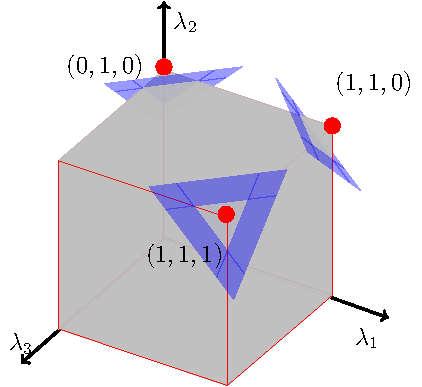
\includegraphics[width=\triplefigure]{\pics/binary/cutForEveryTuple}}
	\subfloat[cut for each complete face]{\label{fig:intb}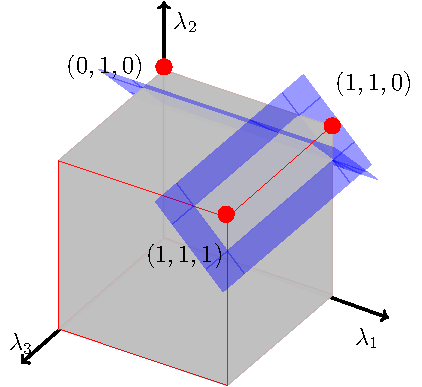
\includegraphics[width=\triplefigure]{\pics/binary/cutForEveryEdge}}
	\subfloat[only one cut]{\label{fig:intc}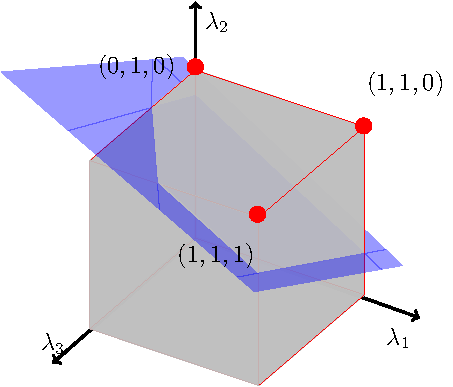
\includegraphics[width=\triplefigure]{\pics/binary/cutForAllTuples}}
	\caption{Exemplification of separating hyperplanes techniques}
	\label{fig:int}
\end{center}
\end{figure}


\begin{rem}
Dimensiunea unei figuri este determinată de argumentul opțional `width'. S-a preferat folosirea de macro-uri (\verb+\singlefigure+ și \verb+\triplefigure+) și nu valori \textquote{hard-coded} datorita flexibilității lor. Shimbând în preambul (în \emph{standard.sty}) valoarea unui astfel de macro se vor schimba automat dimensiunile figurilor ce îl folosesc, fără a mai fi nevoie să se modifice fiecare în parte. \eor
\end{rem}

\subsection{Algoritmi}

În exemplul de mai jos, \algref{alg:run} folosește pachetul \textquote{algorithm2e} pentru redactarea unui algoritm. Prin modificarea opțiunilor din preambulul documentului (în \emph{standard.sty}) este posibilă modificarea structurii/introducerea de noi cuvinte cheie/etc.

\begin{algorithm2e}
\caption{Fault tolerant scheme}
\label{alg:run}
\KwIn{$\mathcal{I}=\mathcal{I}_H(0)\cup \mathcal{I}_F(0);\quad\mathcal{I}_H(0)\neq \emptyset$}
$k \leftarrow$ the current sampling time\;
\ForEach{sensor $i\in \mathcal{I}_F(k-1)$}{
	\If{$r_i(k-1)\in R_i^F$ and $r_i(k) \in R_i^H$}{compute a timer $\bar \theta_i$ \;}
	}
\end{algorithm2e}

\section{Lista bibliografică}

Lista bibliografică este extrasă dintr-un fișier \textquote{*.bib} în care sunt stocate articole/cărți/conferințe în format bibtex (detalii suplimentare pot fi gasite la \url{http://en.wikibooks.org/wiki/LaTeX/Bibliography_Management}). Un exemplu al unei astfel de intrări este:


\begin{verbatim}
@article{gilbert1991linear,
 title={{Linear systems with state and control constraints: the theory and application of maximal output admissible sets}},
 author={Gilbert, EG and Tan, KT},
 journal={IEEE Transactions on Automatic Control},
 volume={36},
 number={9},
 pages={1008--1020},
 year={1991}
}
\end{verbatim}

Pentru citarea în text și listarea intrărilor citate în lista bibliografică s-a folosit pachetul \textquote{biblatex}. În cadrul acestui pachet, cele mai uzuale comenzi de citare sunt următoarele:
\begin{description}[style=nextline]
\item[citare simplă] \verb+\cite{...}+: \cite{bitsoris2006invariance}
\item[citare pusă între paranteze] \verb+\parencite{...}+: \parencite{gilbert1991linear}
\item[citare cu anul pus între paranteze] \verb+\textcite{...}+: \textcite{loechner1999polylib}
\item[citare cu intrări multiple] \verb+\cite{..., ..., ...}+: \cite{bellingham2002receding,garey1979computers,vitus_tunnel-milp:_2008,camponogara2002distributed}
\end{description}

În mod automat, intrările citate în text (și doar ele) vor fi puse în lista de referințe de la sfârșitul manuscrisului.


\section{Localizare: română versus engleză}

În fișierul principal (\emph{thesis.tex}), prin selectarea opțiunii \emph{language=english}, \emph{language=romanian} se poate alterna, respectiv, între formatarea în engleză și cea în română a textului. Câteva exemple sunt:
\begin{itemize}
\item numele cuprins-ului va alterna între \textquote{contents/cuprins}
\item în interiorul listei bibliografice caracterele de legatură se vor adapta (de exemplu, `and' devine `și')
\item \textquote{ghilimelele} se vor adapta la limba folosită (daca pentru a cita un fragment de text folosiți comenzile \verb+\textquote+ sau \verb+\blockquote+)
\item blocurile matematice își vor schimba eticheta, de exemplu `Theorem' devine `Teorema' 
\item referința la un element, de exemplu `Figure 2.3' devine `Figura 2.3'
\end{itemize}

Pentru diacritice (\u a,\^ a,\^ i, \c s, \c t etc.) se poate recurge fie la o codare explicită (\verb+\u a+, \verb+\^ a+, \verb+\^ i+, \verb+\c s+, \verb+\c t+) așa cum e detaliat în \url{http://en.wikibooks.org/wiki/LaTeX/Special_Characters} fie la scrierea lor direct de la o tastatura setată în limba romana într-un editor de text ce suportă utf8.


\section{Diverse}

\begin{description}[style=nextline]
\item[blocuri matematice] pentru blocurile tipic întălnite în matematică (Teoremă, Propoziție, Definiție, Remarcă, etc.) există definiții în preambul ce permit notarea/etichetarea și apelarea lor în mod automat. Spre exemplu, un bloc de tip teoremă se scrie astfel:

\begin{thm}
\label{thm:test}
Conținut teoremă ... urmat de simbolul de terminare a textului. \eot
\end{thm}
\begin{proof}
Demonstrație a afirmațiilor făcute în teoremă.
\end{proof}
Teorema poate fi apoi referită în text prin intermediul etichetei sale: \thmref{thm:test}.
\item[referințe în text]
Cu ajutorul etichetelor asociate blocurilor definite în latex, este posibilă referirea în mod automat a acestor elemente oriunde în manuscris. Prin adaugarea pachetului \emph{hyperref} aceste referințe devin link-uri ce fac legătura cu elementul față de care sunt asociate.
 
Exemple de referințe pot fi ecuații (\eqref{eq:test}), elemente de structură (\chapref{chap:intro}), blocuri matematice (\remref{rem:at}) sau figuri/tabele/algoritmi. Pentru multe dintre acestea,  în fișierele sursă s-au definit macro-uri. Deși nu este obligatoriu, recomandăm uzul acestora datorita flexibilității lor. De exemplu, folosind \verb+\figref{eticheta}+ putem să ne adaptam în mod automat la schimbarea limbajului de lucru (în preambul, acest macro va schimba, în funcție de opțiunea aleasă, între `Figure' și `Figura').

\item[termeni de glosar, acronime]
În fișierul \emph{./cls/gls.tex} introduceți termeni de glosar. Aceștia pot fi apoi folosiți prin apelarea comenzii \verb+\gls{numeTermen}+. Spre exemplu \gls{computer} este un termen de glosar iar \gls{fpsLabel} și \gls{lvm} sunt acronime (atunci când sunt apelate prima oară apar în forma desfășurată, la următorele apelări apar doar cu abreviere: \gls{fpsLabel} și \gls{lvm}). Acești termeni vor fi enumerați într-o listă de termeni de glosar / acronime la începutul lucrării.

Detalii suplimentare pot fi găsite la pagina \url{https://en.wikibooks.org/wiki/LaTeX/Glossary} sau în documentul \url{http://ctan.math.utah.edu/tex-archive/macros/latex/contrib/glossaries/glossariesbegin.pdf}.

\item[fragmente de cod] 
Cu ajutorul pachetului \emph{listings} este posibilă afișarea fragmentelor de cod relevante pentru document prin referirea către un fișier sursă existent (ceea ce înseamnă ca orice modificare a acestuia se va reflecta automat în textul afișat).

Spre exemplu:  în \lstref{lst:s1} este afișat un întreg fișier sursă iar în \lstref{lst:s2} sunt afișate liniile 5-15 din alt fișier sursă folosind comenzile:

%\begin{Verbatim}[samepage=true]
%\lstinputlisting[caption={Cod Matlab -- fișier complet},label={lst:s1}]{\code/s1.m}
%\lstinputlisting[caption={Cod Matlab -- fragment de fișier},label={lst:s2},firstline=5,lastline=15]%{\code/s2.m}
%\end{Verbatim}

\end{description}


\section*{Disclaimer}

Acest ghid de redactare este încă într-o versiune preliminară. Ca atare, diverse erori/bug-uri sunt posibile. Dacă întălniți astfel de situații aduceți-mi-le la cunoștiință la adresa \href{mailto:florin.stoican@acse.pub.ro}{florin.stoican@acse.pub.ro} sau pe forum-ul din cursul asociat lucrării de licență de pe Moodle.
%\chapter{Capitol Test}
\cite{mairal2009online}


%%%%%%%%%%%%%%%%%%%%%% back matter %%%%%%%%%%%%%%%%%%%%%%%%%%%%%%%%%%%%%%
\appendix
\appendixpage
\addappheadtotoc
\begin{appendices}																				  % from here onwards are the appendices
\chapter{Notaţii matematice consacrate}
\label{chap:not}

\begin{description}[style=nextline]
\item[Constante scalare] $\mathrm{a}$, $\mathrm{A}$, $\mathrm{b}$, $\mathrm{B}$, $\mathrm{c}$, $\mathrm{C}$ etc. (litere normale, cu precădere din prima parte a alfabetului);
\item[Constante vectoriale] $\mathbf{a}$, $\mathbf{b}$, $\mathbf{c}$ etc. (litere minuscule, aldine (\textbf{bold}), cu precădere din prima parte a alfabetului);
\item[Constante matriciale] $\mathbf{A}$, $\mathbf{B}$, $\mathbf{C}$, $\mathbf{P}$, $\mathbf{Q}$, $\mathbf{R}$ etc. (litere majuscule, aldine (\textbf{bold}), cu precădere din zona alfabetului unde nu se afl\u a litere alocate în mod tradi\c tional indicilor);
\item[Variabile scalare] $x$, $y$, $z$  etc. (aplecate (\emph{italic}), ne-aldine, cu prec\u adere din ultima parte a alfabetului);
\item[Variabile vectoriale] $\mathbf{x}$, $\mathbf{y}$, $\mathbf{z}$ etc (litere minuscule, aldine (\textbf{bold}), cu precădere din ultima parte a alfabetului);
\item[Variabile  matriciale]  $\mathbf H(q^{-1})$, $\mathbf H(s)$, $\mathbf H(z)$, $\mathbf H(t)$, $\mathbf H[k]$ etc. (litere  majuscule,  aldine (\textbf{bold}), cu unul sau mai multe argumente scalare sau vectoriale);
\item[Operatori]  $\min$ (minim), $\max$ (maxim), opt (optim), $\arg$ opt (argument de optimizare sau punct de optimizare), $q^{-1}$  (întârziere), $Tr$ (urmă (\emph{trace})), $Tz$ (Toeplitz), $Pr$ (proiec\c tie) etc, (litere normale, urmate obligatoriu de explica\c tia privind nota\c tia, la prima utilizare);
\item[Timp continuu] $t\in \mathbb R$;
\item[Timp discret] $n\in \mathbb Z$ sau $k\in \mathbb Z$;
\item[Argument de timp continuu] $(t)$ (între parenteze rotunde);
\item[Argument de timp discret] $[n]$ (între paranteze drepte);
\item[Număr de itera\c tie sau indici] $i$, $j$, $k$, $l$, $m$, $n$  etc. (aplecate, cu precădere din partea de mijloc a alfabetului); exemplu de nota\c tie complex\u a": $x_i^k[n]$ -- componenta $i$ a vectorului $\mathbf x$, la momentul discret $n$, pentru iteratia $k$;
\item[Caractere greceşti frecvent utilizate (în ordinea firească a alfabetului grecesc)]~
\begin{itemize}
\item $\alpha$ (/alfa/, \verb+\alpha+)
\item $\beta$ (/beta/, \verb+\beta+)
\item $\gamma$, $\Gamma$ (/gama/, \verb+\gamma, \Gamma+)
\item $\delta$, $\Delta$ (/delta/, \verb+\delta, \Delta+)
\item $\epsilon$ (/epsilon/, \verb+\epsilon+)
\item $\zeta$ (/\c teta/, \verb+\zeta+)
\item $\eta$ (/ita/, \verb+\eta+)
\item $\theta$, $\Theta$ (/teta/, \verb+\theta, \Theta+)
\item $\kappa$ (/kapa/, \verb+\kappa+)
\item $\lambda$, $\Lambda$ (/lambda/, \verb+\lambda, \Lambda+) a nu se pronun\c ta /lamda/
\item $\mu$ (/miu/, \verb+\mu+)
\item $\nu$ (/niu/, \verb+\nu+)
\item $\xi$ (/xi/, \verb+\xi+)
\item $\pi$, $\Pi$ (/pi/, \verb+\pi, \Pi+)
\item $\rho$ (/ro/, \verb+\rho+)
\item $\sigma$, $\Sigma$ (/sigma/, \verb+\sigma, \Sigma+)
\item $\tau$ (/tau/, \verb+\tau+)
\item $\phi$, $\varphi$, $\Phi$ (/fi/, \verb+\phi, \varphi, \Phi+)
\item $\chi$ (/hi/, \verb+\chi+)
\item $\psi$, $\Psi$ (/psi/, \verb+\psi, \Psi+)
\item $\omega$, $\Omega$ (/omega/, \verb+\omega, \Omega+)
\end{itemize}
Şi  în  cazul  lor,  se  vor  respecta  regulile  de  nota\c tie  pentru  scalari/vectori. % Totuşi,  în  cazul scalarilor, se recomandă ca literele să nu fie scrise aplecat. De exemplu, se va prefera  $\mathrm \alpha$ şi nu $\alpha$.
\item[Alte nota\c tii unificate în Automatică]~
\begin{description}[before={\renewcommand\makelabel[1]{##1 =}},leftmargin=!,labelwidth=\widthof{\bfseries blaaaaaaaa}]
\item[$J$, $\mathbf J$] criteriu (de optimizare), func\c tie-criteriu, (func\c tie) cost, func\c tie economică, func\c tie obiectiv
\item[$u$, $\mathbf u$] intrarea/comanda (scalară sau vectorială a) unui sistem dinamic
\item[$x$, $\mathbf x$] starea (scalară sau vectorială a) unui sistem dinamic
\item[$y$, $\mathbf y$] ieşirea (scalară sau vectorială a) unui sistem dinamic
\item[$v$, $\mathbf v$] perturba\c tia exogenă (scalară sau vectorială) a unui sistem dinamic (asociată cu ieşirile)
\item[$w$, $\mathbf w$] perturba\c tia endogenă (scalară sau vectorială) a unui sistem dinamic (asociată cu stările)
\item[$e$, $\mathbf e$] zgomotul alb (scalar sau vectorial)
\item[$\mathrm{e}$] numărul lui Nepper, baza logaritmului natural (se scrie drept şi nu aplecat)
\item[$s$] variabila (complexă) Laplace
\item[$z$] variabila complexă circulară (specifică Transformatei Z)
\item[$f$, $\mathbf f$] func\c tie neliniară (scalară sau vectorială) asociată în special ecua\c tiei de stare
\item[$g$, $\mathbf g$] func\c tie neliniară (scalară sau vectorială) asociată în special ecua\c tiei de ieşire
\item[$\nabla$, $\nabla_x$] operatorul  de  gradient/Jacobian  (se  pronun\c tă  /nabla/;  \verb+\nabla+);  acest operator se poate nota şi prin $\mathbf J_x$
\item[$\Diamond$, $\Diamond_x$] operatorul  Hessian (se  pronun\c tă  /romb/;  \verb+\Diamond+);  acest operator se poate nota şi prin $\mathbf J_{xx}$
\item[$\mathbf A^T$] transpusa matricii $\mathbf A$
\item[$\bar{\mathbf A}$] conjugata complex\u a a matricii $\mathbf A$
\item[$\bar{\mathbf A}^T$, $A^*$] transpusa  şi  conjugata  complexă  a  matricii $\mathbf A$   (\emph{hermitica}  acesteia);  a  doua nota\c tie poate fi folosită şi pentru a indica doar conjugarea complexă, cu condi\c tia să se men\c tioneze clar de la început semnifica\c tia acesteia
\item[$\mathbf v^R$]  versiunea răsturnată a vectorului  $\mathbf v$  (adică rearanjată prin citirea de jos în sus)
\end{description}
\end{description}
% fisiere sursa

\chapter{Fișiere sursă}
\label{chap:sources}

\lstinputlisting[caption={Cod Matlab -- fișier complet},label={lst:s1}]{\code/s1.m}
\lstinputlisting[caption={Cod Matlab -- fragment de fișier},label={lst:s2},firstline=5,lastline=15]{\code/s2.m}
\end{appendices}

\cleardoublepage

\printbibliography[heading=bibintoc]
\end{document}